\newcommand\sh{$^\sharp$}

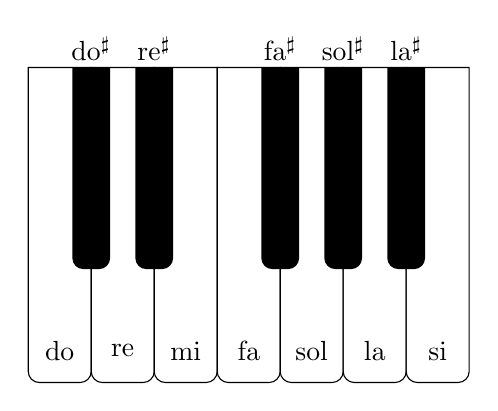
\begin{tikzpicture}[scale=.8]

  \foreach \i in {0,...,6} {
    \draw
         (\i,       5)
      -- ({\i + 1}, 5)
      {[rounded corners]
        -- ({\i + 1}, 0)
        -- (\i,       0)
      }
      -- cycle;
  }
  \foreach\i in {1,2,4,5,6} {
    \fill[black]
         ({\i + .3}, 5.0)
      -- ({\i - .3}, 5.0)
      {[rounded corners]
        -- ({\i - .3}, 1.8)
        -- ({\i + .3}, 1.8)
      }
      -- cycle;
  }

  \node at (0.5, .5) {do};  \node at (1, 5.3) {do\sh};
  \node at (1.5, .5) {re};  \node at (2, 5.3) {re\sh};
  \node at (2.5, .5) {mi};
  \node at (3.5, .5) {fa};  \node at (4, 5.3) {fa\sh};
  \node at (4.5, .5) {sol}; \node at (5, 5.3) {sol\sh};
  \node at (5.5, .5) {la};  \node at (6, 5.3) {la\sh};
  \node at (6.5, .5) {si};

\end{tikzpicture}

